\documentclass[twoside]{book}

% Packages required by doxygen
\usepackage{fixltx2e}
\usepackage{calc}
\usepackage{doxygen}
\usepackage[export]{adjustbox} % also loads graphicx
\usepackage{graphicx}
\usepackage[utf8]{inputenc}
\usepackage{makeidx}
\usepackage{multicol}
\usepackage{multirow}
\PassOptionsToPackage{warn}{textcomp}
\usepackage{textcomp}
\usepackage[nointegrals]{wasysym}
\usepackage[table]{xcolor}

% Font selection
\usepackage[T1]{fontenc}
\usepackage[scaled=.90]{helvet}
\usepackage{courier}
\usepackage{amssymb}
\usepackage{sectsty}
\renewcommand{\familydefault}{\sfdefault}
\allsectionsfont{%
  \fontseries{bc}\selectfont%
  \color{darkgray}%
}
\renewcommand{\DoxyLabelFont}{%
  \fontseries{bc}\selectfont%
  \color{darkgray}%
}
\newcommand{\+}{\discretionary{\mbox{\scriptsize$\hookleftarrow$}}{}{}}

% Page & text layout
\usepackage{geometry}
\geometry{%
  a4paper,%
  top=2.5cm,%
  bottom=2.5cm,%
  left=2.5cm,%
  right=2.5cm%
}
\tolerance=750
\hfuzz=15pt
\hbadness=750
\setlength{\emergencystretch}{15pt}
\setlength{\parindent}{0cm}
\setlength{\parskip}{3ex plus 2ex minus 2ex}
\makeatletter
\renewcommand{\paragraph}{%
  \@startsection{paragraph}{4}{0ex}{-1.0ex}{1.0ex}{%
    \normalfont\normalsize\bfseries\SS@parafont%
  }%
}
\renewcommand{\subparagraph}{%
  \@startsection{subparagraph}{5}{0ex}{-1.0ex}{1.0ex}{%
    \normalfont\normalsize\bfseries\SS@subparafont%
  }%
}
\makeatother

% Headers & footers
\usepackage{fancyhdr}
\pagestyle{fancyplain}
\fancyhead[LE]{\fancyplain{}{\bfseries\thepage}}
\fancyhead[CE]{\fancyplain{}{}}
\fancyhead[RE]{\fancyplain{}{\bfseries\leftmark}}
\fancyhead[LO]{\fancyplain{}{\bfseries\rightmark}}
\fancyhead[CO]{\fancyplain{}{}}
\fancyhead[RO]{\fancyplain{}{\bfseries\thepage}}
\fancyfoot[LE]{\fancyplain{}{}}
\fancyfoot[CE]{\fancyplain{}{}}
\fancyfoot[RE]{\fancyplain{}{\bfseries\scriptsize Generated by Doxygen }}
\fancyfoot[LO]{\fancyplain{}{\bfseries\scriptsize Generated by Doxygen }}
\fancyfoot[CO]{\fancyplain{}{}}
\fancyfoot[RO]{\fancyplain{}{}}
\renewcommand{\footrulewidth}{0.4pt}
\renewcommand{\chaptermark}[1]{%
  \markboth{#1}{}%
}
\renewcommand{\sectionmark}[1]{%
  \markright{\thesection\ #1}%
}

% Indices & bibliography
\usepackage{natbib}
\usepackage[titles]{tocloft}
\setcounter{tocdepth}{3}
\setcounter{secnumdepth}{5}
\makeindex

% Hyperlinks (required, but should be loaded last)
\usepackage{ifpdf}
\ifpdf
  \usepackage[pdftex,pagebackref=true]{hyperref}
\else
  \usepackage[ps2pdf,pagebackref=true]{hyperref}
\fi
\hypersetup{%
  colorlinks=true,%
  linkcolor=blue,%
  citecolor=blue,%
  unicode%
}

% Custom commands
\newcommand{\clearemptydoublepage}{%
  \newpage{\pagestyle{empty}\cleardoublepage}%
}

\usepackage{caption}
\captionsetup{labelsep=space,justification=centering,font={bf},singlelinecheck=off,skip=4pt,position=top}

%===== C O N T E N T S =====

\begin{document}

% Titlepage & ToC
\hypersetup{pageanchor=false,
             bookmarksnumbered=true,
             pdfencoding=unicode
            }
\pagenumbering{roman}
\begin{titlepage}
\vspace*{7cm}
\begin{center}%
{\Large Colorado\+\_\+\+Alarm\+\_\+\+Clock }\\
\vspace*{1cm}
{\large Generated by Doxygen 1.8.11}\\
\end{center}
\end{titlepage}
\clearemptydoublepage
\tableofcontents
\clearemptydoublepage
\pagenumbering{arabic}
\hypersetup{pageanchor=true}

%--- Begin generated contents ---
\chapter{Hierarchical Index}
\section{Class Hierarchy}
This inheritance list is sorted roughly, but not completely, alphabetically\+:\begin{DoxyCompactList}
\item \contentsline{section}{com.\+robobrandon.\+simpleweather.\+Weather\+Pull\+Service}{\pageref{classcom_1_1robobrandon_1_1simpleweather_1_1_weather_pull_service}}{}
\item Activity\begin{DoxyCompactList}
\item \contentsline{section}{com.\+robobrandon.\+simpleweather.\+Alarm\+Activity}{\pageref{classcom_1_1robobrandon_1_1simpleweather_1_1_alarm_activity}}{}
\item \contentsline{section}{com.\+robobrandon.\+simpleweather.\+Main\+Activity}{\pageref{classcom_1_1robobrandon_1_1simpleweather_1_1_main_activity}}{}
\end{DoxyCompactList}
\item Application\begin{DoxyCompactList}
\item \contentsline{section}{com.\+robobrandon.\+simpleweather.\+Mars\+Weather}{\pageref{classcom_1_1robobrandon_1_1simpleweather_1_1_mars_weather}}{}
\end{DoxyCompactList}
\item Intent\+Service\begin{DoxyCompactList}
\item \contentsline{section}{com.\+robobrandon.\+simpleweather.\+Alarm\+Service}{\pageref{classcom_1_1robobrandon_1_1simpleweather_1_1_alarm_service}}{}
\end{DoxyCompactList}
\item Json\+Object\+Request\begin{DoxyCompactList}
\item \contentsline{section}{com.\+robobrandon.\+simpleweather.\+Custom\+Json\+Request}{\pageref{classcom_1_1robobrandon_1_1simpleweather_1_1_custom_json_request}}{}
\end{DoxyCompactList}
\item Wakeful\+Broadcast\+Receiver\begin{DoxyCompactList}
\item \contentsline{section}{com.\+robobrandon.\+simpleweather.\+Alarm\+Receiver}{\pageref{classcom_1_1robobrandon_1_1simpleweather_1_1_alarm_receiver}}{}
\end{DoxyCompactList}
\end{DoxyCompactList}

\chapter{Class Index}
\section{Class List}
Here are the classes, structs, unions and interfaces with brief descriptions\+:\begin{DoxyCompactList}
\item\contentsline{section}{\hyperlink{classcom_1_1robobrandon_1_1simpleweather_1_1_alarm_activity}{com.\+robobrandon.\+simpleweather.\+Alarm\+Activity} }{\pageref{classcom_1_1robobrandon_1_1simpleweather_1_1_alarm_activity}}{}
\item\contentsline{section}{\hyperlink{classcom_1_1robobrandon_1_1simpleweather_1_1_alarm_receiver}{com.\+robobrandon.\+simpleweather.\+Alarm\+Receiver} }{\pageref{classcom_1_1robobrandon_1_1simpleweather_1_1_alarm_receiver}}{}
\item\contentsline{section}{\hyperlink{classcom_1_1robobrandon_1_1simpleweather_1_1_alarm_service}{com.\+robobrandon.\+simpleweather.\+Alarm\+Service} }{\pageref{classcom_1_1robobrandon_1_1simpleweather_1_1_alarm_service}}{}
\item\contentsline{section}{\hyperlink{classcom_1_1robobrandon_1_1simpleweather_1_1_custom_json_request}{com.\+robobrandon.\+simpleweather.\+Custom\+Json\+Request} }{\pageref{classcom_1_1robobrandon_1_1simpleweather_1_1_custom_json_request}}{}
\item\contentsline{section}{\hyperlink{classcom_1_1robobrandon_1_1simpleweather_1_1_main_activity}{com.\+robobrandon.\+simpleweather.\+Main\+Activity} }{\pageref{classcom_1_1robobrandon_1_1simpleweather_1_1_main_activity}}{}
\item\contentsline{section}{\hyperlink{classcom_1_1robobrandon_1_1simpleweather_1_1_mars_weather}{com.\+robobrandon.\+simpleweather.\+Mars\+Weather} }{\pageref{classcom_1_1robobrandon_1_1simpleweather_1_1_mars_weather}}{}
\item\contentsline{section}{\hyperlink{classcom_1_1robobrandon_1_1simpleweather_1_1_weather_pull_service}{com.\+robobrandon.\+simpleweather.\+Weather\+Pull\+Service} }{\pageref{classcom_1_1robobrandon_1_1simpleweather_1_1_weather_pull_service}}{}
\end{DoxyCompactList}

\chapter{Class Documentation}
\hypertarget{classcom_1_1robobrandon_1_1simpleweather_1_1_alarm_activity}{}\section{com.\+robobrandon.\+simpleweather.\+Alarm\+Activity Class Reference}
\label{classcom_1_1robobrandon_1_1simpleweather_1_1_alarm_activity}\index{com.\+robobrandon.\+simpleweather.\+Alarm\+Activity@{com.\+robobrandon.\+simpleweather.\+Alarm\+Activity}}
Inheritance diagram for com.\+robobrandon.\+simpleweather.\+Alarm\+Activity\+:\begin{figure}[H]
\begin{center}
\leavevmode
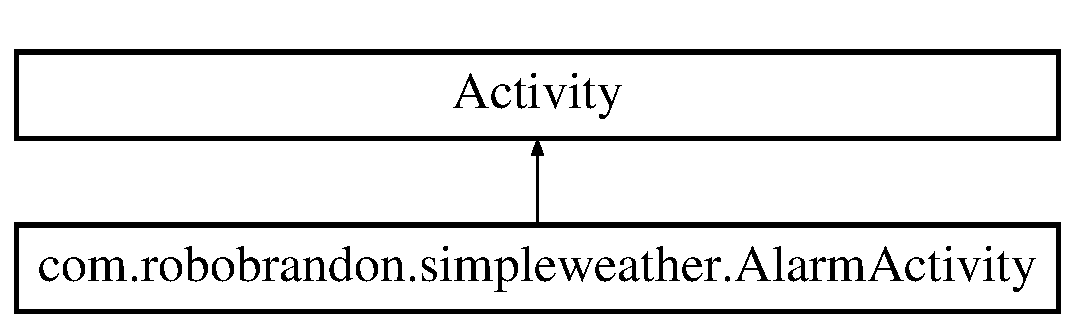
\includegraphics[height=2.000000cm]{classcom_1_1robobrandon_1_1simpleweather_1_1_alarm_activity}
\end{center}
\end{figure}
\subsection*{Public Member Functions}
\begin{DoxyCompactItemize}
\item 
void {\bfseries on\+Start} ()\hypertarget{classcom_1_1robobrandon_1_1simpleweather_1_1_alarm_activity_aca2a5b30d11445f041110b56360e6828}{}\label{classcom_1_1robobrandon_1_1simpleweather_1_1_alarm_activity_aca2a5b30d11445f041110b56360e6828}

\item 
void {\bfseries on\+Toggle\+Clicked} (View view)\hypertarget{classcom_1_1robobrandon_1_1simpleweather_1_1_alarm_activity_a50907175c76e1f6ef2123b789973fa5f}{}\label{classcom_1_1robobrandon_1_1simpleweather_1_1_alarm_activity_a50907175c76e1f6ef2123b789973fa5f}

\item 
void {\bfseries set\+Alarm\+Text} (String alarm\+Text)\hypertarget{classcom_1_1robobrandon_1_1simpleweather_1_1_alarm_activity_a8f3e21e53d2b2ef4df07c738bbbe2ae4}{}\label{classcom_1_1robobrandon_1_1simpleweather_1_1_alarm_activity_a8f3e21e53d2b2ef4df07c738bbbe2ae4}

\end{DoxyCompactItemize}
\subsection*{Static Public Member Functions}
\begin{DoxyCompactItemize}
\item 
static \hyperlink{classcom_1_1robobrandon_1_1simpleweather_1_1_alarm_activity}{Alarm\+Activity} {\bfseries instance} ()\hypertarget{classcom_1_1robobrandon_1_1simpleweather_1_1_alarm_activity_a93c95929b6be5ab9ed665157dfd9cf2f}{}\label{classcom_1_1robobrandon_1_1simpleweather_1_1_alarm_activity_a93c95929b6be5ab9ed665157dfd9cf2f}

\end{DoxyCompactItemize}
\subsection*{Protected Member Functions}
\begin{DoxyCompactItemize}
\item 
void {\bfseries on\+Create} (Bundle saved\+Instance\+State)\hypertarget{classcom_1_1robobrandon_1_1simpleweather_1_1_alarm_activity_af2a8ca46bb30a0ad2bfa87f43cda7b64}{}\label{classcom_1_1robobrandon_1_1simpleweather_1_1_alarm_activity_af2a8ca46bb30a0ad2bfa87f43cda7b64}

\end{DoxyCompactItemize}
\subsection*{Private Attributes}
\begin{DoxyCompactItemize}
\item 
Pending\+Intent {\bfseries pending\+Intent}\hypertarget{classcom_1_1robobrandon_1_1simpleweather_1_1_alarm_activity_af48c1894df3be4b19244cbc7cc081edb}{}\label{classcom_1_1robobrandon_1_1simpleweather_1_1_alarm_activity_af48c1894df3be4b19244cbc7cc081edb}

\item 
Time\+Picker {\bfseries alarm\+Time\+Picker}\hypertarget{classcom_1_1robobrandon_1_1simpleweather_1_1_alarm_activity_a053ab29c0b7302964ceabe1d91cf1f28}{}\label{classcom_1_1robobrandon_1_1simpleweather_1_1_alarm_activity_a053ab29c0b7302964ceabe1d91cf1f28}

\item 
Text\+View {\bfseries alarm\+Text\+View}\hypertarget{classcom_1_1robobrandon_1_1simpleweather_1_1_alarm_activity_a29352fb3b8105b5703bf36ef938f33ad}{}\label{classcom_1_1robobrandon_1_1simpleweather_1_1_alarm_activity_a29352fb3b8105b5703bf36ef938f33ad}

\end{DoxyCompactItemize}
\subsection*{Static Private Attributes}
\begin{DoxyCompactItemize}
\item 
static \hyperlink{classcom_1_1robobrandon_1_1simpleweather_1_1_alarm_activity}{Alarm\+Activity} {\bfseries inst}\hypertarget{classcom_1_1robobrandon_1_1simpleweather_1_1_alarm_activity_aaa38485817f057c8bab7d74d020cf424}{}\label{classcom_1_1robobrandon_1_1simpleweather_1_1_alarm_activity_aaa38485817f057c8bab7d74d020cf424}

\end{DoxyCompactItemize}


The documentation for this class was generated from the following file\+:\begin{DoxyCompactItemize}
\item 
C\+:/\+Users/\+Amir/\+Android\+Studio\+Projects/colorado\+\_\+alarm/app/src/main/java/com/robobrandon/simpleweather/Alarm\+Activity.\+java\end{DoxyCompactItemize}

\hypertarget{classcom_1_1robobrandon_1_1simpleweather_1_1_alarm_receiver}{}\section{com.\+robobrandon.\+simpleweather.\+Alarm\+Receiver Class Reference}
\label{classcom_1_1robobrandon_1_1simpleweather_1_1_alarm_receiver}\index{com.\+robobrandon.\+simpleweather.\+Alarm\+Receiver@{com.\+robobrandon.\+simpleweather.\+Alarm\+Receiver}}
Inheritance diagram for com.\+robobrandon.\+simpleweather.\+Alarm\+Receiver\+:\begin{figure}[H]
\begin{center}
\leavevmode
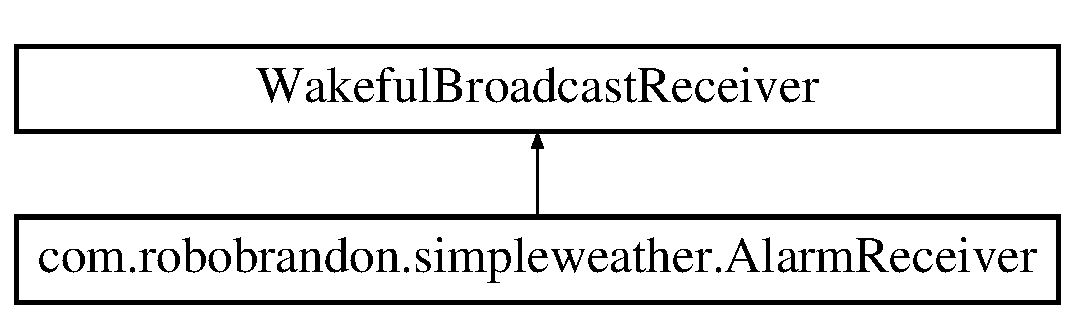
\includegraphics[height=2.000000cm]{classcom_1_1robobrandon_1_1simpleweather_1_1_alarm_receiver}
\end{center}
\end{figure}
\subsection*{Public Member Functions}
\begin{DoxyCompactItemize}
\item 
void {\bfseries on\+Receive} (final Context context, Intent intent)\hypertarget{classcom_1_1robobrandon_1_1simpleweather_1_1_alarm_receiver_a8fa7ba715ef9f140ab59df03bc9d66ae}{}\label{classcom_1_1robobrandon_1_1simpleweather_1_1_alarm_receiver_a8fa7ba715ef9f140ab59df03bc9d66ae}

\end{DoxyCompactItemize}


The documentation for this class was generated from the following file\+:\begin{DoxyCompactItemize}
\item 
C\+:/\+Users/\+Amir/\+Android\+Studio\+Projects/colorado\+\_\+alarm/app/src/main/java/com/robobrandon/simpleweather/Alarm\+Receiver.\+java\end{DoxyCompactItemize}

\hypertarget{classcom_1_1robobrandon_1_1simpleweather_1_1_alarm_service}{}\section{com.\+robobrandon.\+simpleweather.\+Alarm\+Service Class Reference}
\label{classcom_1_1robobrandon_1_1simpleweather_1_1_alarm_service}\index{com.\+robobrandon.\+simpleweather.\+Alarm\+Service@{com.\+robobrandon.\+simpleweather.\+Alarm\+Service}}
Inheritance diagram for com.\+robobrandon.\+simpleweather.\+Alarm\+Service\+:\begin{figure}[H]
\begin{center}
\leavevmode
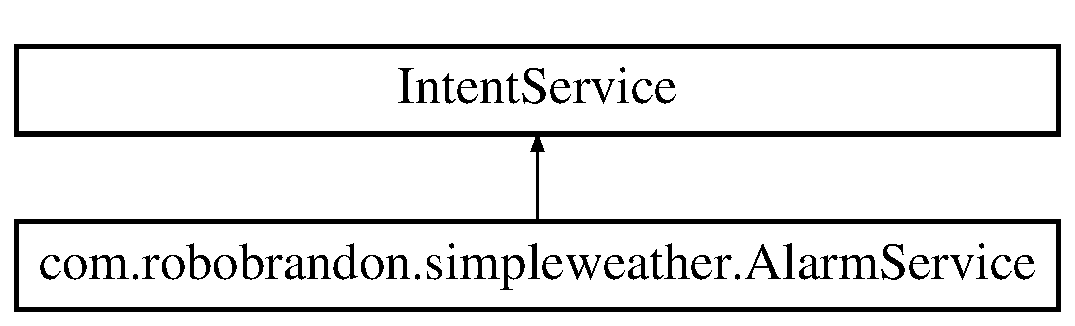
\includegraphics[height=2.000000cm]{classcom_1_1robobrandon_1_1simpleweather_1_1_alarm_service}
\end{center}
\end{figure}
\subsection*{Public Member Functions}
\begin{DoxyCompactItemize}
\item 
void {\bfseries on\+Handle\+Intent} (Intent intent)\hypertarget{classcom_1_1robobrandon_1_1simpleweather_1_1_alarm_service_a2a2bebc18c00a0de0a18cd2c4e912537}{}\label{classcom_1_1robobrandon_1_1simpleweather_1_1_alarm_service_a2a2bebc18c00a0de0a18cd2c4e912537}

\end{DoxyCompactItemize}
\subsection*{Private Member Functions}
\begin{DoxyCompactItemize}
\item 
void {\bfseries send\+Notification} (String msg)\hypertarget{classcom_1_1robobrandon_1_1simpleweather_1_1_alarm_service_a054f4f065a13580922c9cadfe1534e64}{}\label{classcom_1_1robobrandon_1_1simpleweather_1_1_alarm_service_a054f4f065a13580922c9cadfe1534e64}

\end{DoxyCompactItemize}
\subsection*{Private Attributes}
\begin{DoxyCompactItemize}
\item 
Notification\+Manager {\bfseries alarm\+Notification\+Manager}\hypertarget{classcom_1_1robobrandon_1_1simpleweather_1_1_alarm_service_a6f91d2b5874de28aac899354af70fb3f}{}\label{classcom_1_1robobrandon_1_1simpleweather_1_1_alarm_service_a6f91d2b5874de28aac899354af70fb3f}

\end{DoxyCompactItemize}


The documentation for this class was generated from the following file\+:\begin{DoxyCompactItemize}
\item 
C\+:/\+Users/\+Amir/\+Android\+Studio\+Projects/colorado\+\_\+alarm/app/src/main/java/com/robobrandon/simpleweather/Alarm\+Service.\+java\end{DoxyCompactItemize}

\hypertarget{classcom_1_1robobrandon_1_1simpleweather_1_1_custom_json_request}{}\section{com.\+robobrandon.\+simpleweather.\+Custom\+Json\+Request Class Reference}
\label{classcom_1_1robobrandon_1_1simpleweather_1_1_custom_json_request}\index{com.\+robobrandon.\+simpleweather.\+Custom\+Json\+Request@{com.\+robobrandon.\+simpleweather.\+Custom\+Json\+Request}}
Inheritance diagram for com.\+robobrandon.\+simpleweather.\+Custom\+Json\+Request\+:\begin{figure}[H]
\begin{center}
\leavevmode
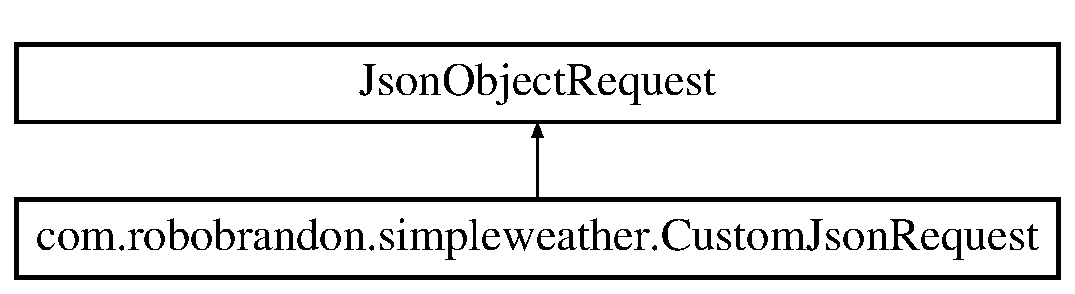
\includegraphics[height=2.000000cm]{classcom_1_1robobrandon_1_1simpleweather_1_1_custom_json_request}
\end{center}
\end{figure}
\subsection*{Public Member Functions}
\begin{DoxyCompactItemize}
\item 
{\bfseries Custom\+Json\+Request} (int method, String url, J\+S\+O\+N\+Object json\+Request, Response.\+Listener$<$ J\+S\+O\+N\+Object $>$ listener, Response.\+Error\+Listener error\+Listener)\hypertarget{classcom_1_1robobrandon_1_1simpleweather_1_1_custom_json_request_a67eb09303e897e4ab90f8ff2388482a6}{}\label{classcom_1_1robobrandon_1_1simpleweather_1_1_custom_json_request_a67eb09303e897e4ab90f8ff2388482a6}

\item 
void {\bfseries set\+Priority} (Priority priority)\hypertarget{classcom_1_1robobrandon_1_1simpleweather_1_1_custom_json_request_a40feb1f46a5a0ce8afdb77c40e8ff0c6}{}\label{classcom_1_1robobrandon_1_1simpleweather_1_1_custom_json_request_a40feb1f46a5a0ce8afdb77c40e8ff0c6}

\item 
Priority {\bfseries get\+Priority} ()\hypertarget{classcom_1_1robobrandon_1_1simpleweather_1_1_custom_json_request_a86527c5df85ea0adca79da6b98b64713}{}\label{classcom_1_1robobrandon_1_1simpleweather_1_1_custom_json_request_a86527c5df85ea0adca79da6b98b64713}

\end{DoxyCompactItemize}
\subsection*{Private Attributes}
\begin{DoxyCompactItemize}
\item 
Priority {\bfseries m\+Priority}\hypertarget{classcom_1_1robobrandon_1_1simpleweather_1_1_custom_json_request_a6f67cf51f22bab671dd1fb10d2acfa2d}{}\label{classcom_1_1robobrandon_1_1simpleweather_1_1_custom_json_request_a6f67cf51f22bab671dd1fb10d2acfa2d}

\end{DoxyCompactItemize}


The documentation for this class was generated from the following file\+:\begin{DoxyCompactItemize}
\item 
C\+:/\+Users/\+Amir/\+Android\+Studio\+Projects/colorado\+\_\+alarm/app/src/main/java/com/robobrandon/simpleweather/Custom\+Json\+Request.\+java\end{DoxyCompactItemize}

\hypertarget{classcom_1_1robobrandon_1_1simpleweather_1_1_main_activity}{}\section{com.\+robobrandon.\+simpleweather.\+Main\+Activity Class Reference}
\label{classcom_1_1robobrandon_1_1simpleweather_1_1_main_activity}\index{com.\+robobrandon.\+simpleweather.\+Main\+Activity@{com.\+robobrandon.\+simpleweather.\+Main\+Activity}}
Inheritance diagram for com.\+robobrandon.\+simpleweather.\+Main\+Activity\+:\begin{figure}[H]
\begin{center}
\leavevmode
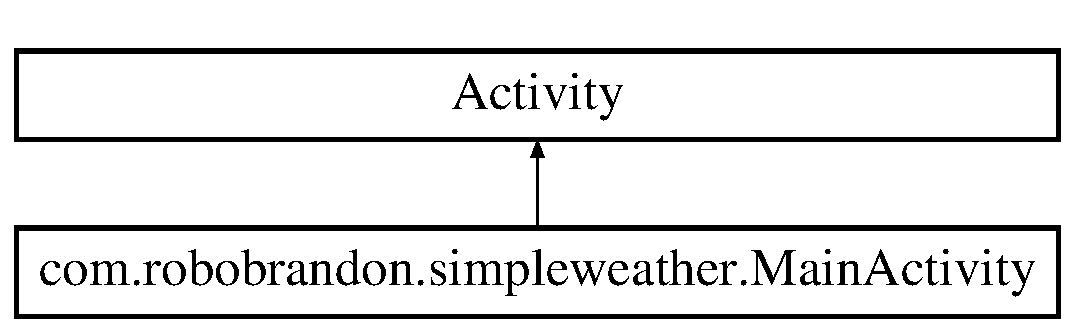
\includegraphics[height=2.000000cm]{classcom_1_1robobrandon_1_1simpleweather_1_1_main_activity}
\end{center}
\end{figure}
\subsection*{Public Member Functions}
\begin{DoxyCompactItemize}
\item 
void {\bfseries set\+Alarm} (View view)\hypertarget{classcom_1_1robobrandon_1_1simpleweather_1_1_main_activity_a0f986012e87d895c48714f2a693f7da9}{}\label{classcom_1_1robobrandon_1_1simpleweather_1_1_main_activity_a0f986012e87d895c48714f2a693f7da9}

\end{DoxyCompactItemize}
\subsection*{Protected Member Functions}
\begin{DoxyCompactItemize}
\item 
void {\bfseries on\+Create} (Bundle saved\+Instance\+State)\hypertarget{classcom_1_1robobrandon_1_1simpleweather_1_1_main_activity_a23ca305fadf606da706cf407937ceee7}{}\label{classcom_1_1robobrandon_1_1simpleweather_1_1_main_activity_a23ca305fadf606da706cf407937ceee7}

\item 
void {\bfseries on\+Stop} ()\hypertarget{classcom_1_1robobrandon_1_1simpleweather_1_1_main_activity_a342fdaa768a8cf6fc71d6f1e30a4209a}{}\label{classcom_1_1robobrandon_1_1simpleweather_1_1_main_activity_a342fdaa768a8cf6fc71d6f1e30a4209a}

\end{DoxyCompactItemize}
\subsection*{Private Member Functions}
\begin{DoxyCompactItemize}
\item 
void \hyperlink{classcom_1_1robobrandon_1_1simpleweather_1_1_main_activity_aa749eb4949c20efc608a0b11fa9a37f4}{search\+Random\+Image} ()  throws Exception 
\item 
void \hyperlink{classcom_1_1robobrandon_1_1simpleweather_1_1_main_activity_abdc4cd0a49c58fc47eaf041372ed331e}{load\+Img} (String image\+Url)
\item 
void \hyperlink{classcom_1_1robobrandon_1_1simpleweather_1_1_main_activity_aa63758c27d84a822f308d5508907ebcc}{load\+Weather\+Data} ()
\item 
void {\bfseries image\+Error} (Exception e)\hypertarget{classcom_1_1robobrandon_1_1simpleweather_1_1_main_activity_a0b4e8a6f728c338118174a2e7dafd5a7}{}\label{classcom_1_1robobrandon_1_1simpleweather_1_1_main_activity_a0b4e8a6f728c338118174a2e7dafd5a7}

\item 
void {\bfseries txt\+Error} (Exception e)\hypertarget{classcom_1_1robobrandon_1_1simpleweather_1_1_main_activity_a1746a82e6ba67d8cfbb077714b7b17eb}{}\label{classcom_1_1robobrandon_1_1simpleweather_1_1_main_activity_a1746a82e6ba67d8cfbb077714b7b17eb}

\end{DoxyCompactItemize}


\subsection{Member Function Documentation}
\index{com\+::robobrandon\+::simpleweather\+::\+Main\+Activity@{com\+::robobrandon\+::simpleweather\+::\+Main\+Activity}!load\+Img@{load\+Img}}
\index{load\+Img@{load\+Img}!com\+::robobrandon\+::simpleweather\+::\+Main\+Activity@{com\+::robobrandon\+::simpleweather\+::\+Main\+Activity}}
\subsubsection[{\texorpdfstring{load\+Img(\+String image\+Url)}{loadImg(String imageUrl)}}]{\setlength{\rightskip}{0pt plus 5cm}void com.\+robobrandon.\+simpleweather.\+Main\+Activity.\+load\+Img (
\begin{DoxyParamCaption}
\item[{String}]{image\+Url}
\end{DoxyParamCaption}
)\hspace{0.3cm}{\ttfamily [private]}}\hypertarget{classcom_1_1robobrandon_1_1simpleweather_1_1_main_activity_abdc4cd0a49c58fc47eaf041372ed331e}{}\label{classcom_1_1robobrandon_1_1simpleweather_1_1_main_activity_abdc4cd0a49c58fc47eaf041372ed331e}
Downloads and displays the picture using Volley. 
\begin{DoxyParams}{Parameters}
{\em image\+Url} & the U\+RL of the picture. \\
\hline
\end{DoxyParams}
\index{com\+::robobrandon\+::simpleweather\+::\+Main\+Activity@{com\+::robobrandon\+::simpleweather\+::\+Main\+Activity}!load\+Weather\+Data@{load\+Weather\+Data}}
\index{load\+Weather\+Data@{load\+Weather\+Data}!com\+::robobrandon\+::simpleweather\+::\+Main\+Activity@{com\+::robobrandon\+::simpleweather\+::\+Main\+Activity}}
\subsubsection[{\texorpdfstring{load\+Weather\+Data()}{loadWeatherData()}}]{\setlength{\rightskip}{0pt plus 5cm}void com.\+robobrandon.\+simpleweather.\+Main\+Activity.\+load\+Weather\+Data (
\begin{DoxyParamCaption}
{}
\end{DoxyParamCaption}
)\hspace{0.3cm}{\ttfamily [private]}}\hypertarget{classcom_1_1robobrandon_1_1simpleweather_1_1_main_activity_aa63758c27d84a822f308d5508907ebcc}{}\label{classcom_1_1robobrandon_1_1simpleweather_1_1_main_activity_aa63758c27d84a822f308d5508907ebcc}
Fetches and displays the weather data of Mars. \index{com\+::robobrandon\+::simpleweather\+::\+Main\+Activity@{com\+::robobrandon\+::simpleweather\+::\+Main\+Activity}!search\+Random\+Image@{search\+Random\+Image}}
\index{search\+Random\+Image@{search\+Random\+Image}!com\+::robobrandon\+::simpleweather\+::\+Main\+Activity@{com\+::robobrandon\+::simpleweather\+::\+Main\+Activity}}
\subsubsection[{\texorpdfstring{search\+Random\+Image()}{searchRandomImage()}}]{\setlength{\rightskip}{0pt plus 5cm}void com.\+robobrandon.\+simpleweather.\+Main\+Activity.\+search\+Random\+Image (
\begin{DoxyParamCaption}
{}
\end{DoxyParamCaption}
) throws Exception\hspace{0.3cm}{\ttfamily [private]}}\hypertarget{classcom_1_1robobrandon_1_1simpleweather_1_1_main_activity_aa749eb4949c20efc608a0b11fa9a37f4}{}\label{classcom_1_1robobrandon_1_1simpleweather_1_1_main_activity_aa749eb4949c20efc608a0b11fa9a37f4}
Fetches a random picture of Mars, using Flickr A\+P\+Is, and then displays it. 
\begin{DoxyExceptions}{Exceptions}
{\em Exception} & When a working A\+PI key is not provided. \\
\hline
\end{DoxyExceptions}


The documentation for this class was generated from the following file\+:\begin{DoxyCompactItemize}
\item 
C\+:/\+Users/\+Amir/\+Android\+Studio\+Projects/colorado\+\_\+alarm/app/src/main/java/com/robobrandon/simpleweather/Main\+Activity.\+java\end{DoxyCompactItemize}

\hypertarget{classcom_1_1robobrandon_1_1simpleweather_1_1_mars_weather}{}\section{com.\+robobrandon.\+simpleweather.\+Mars\+Weather Class Reference}
\label{classcom_1_1robobrandon_1_1simpleweather_1_1_mars_weather}\index{com.\+robobrandon.\+simpleweather.\+Mars\+Weather@{com.\+robobrandon.\+simpleweather.\+Mars\+Weather}}
Inheritance diagram for com.\+robobrandon.\+simpleweather.\+Mars\+Weather\+:\begin{figure}[H]
\begin{center}
\leavevmode
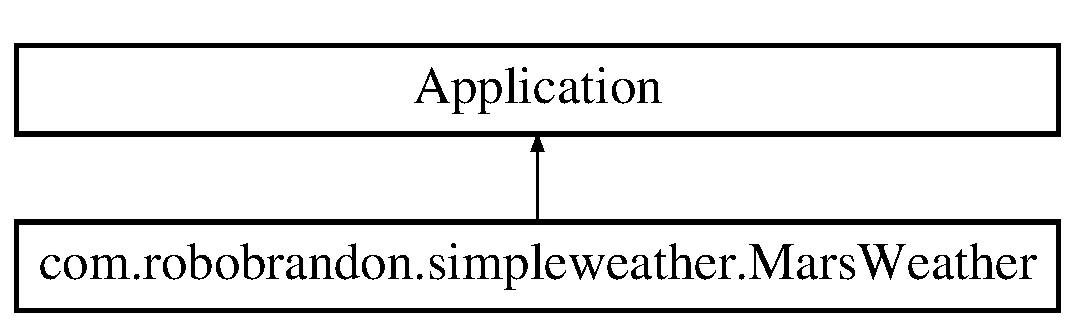
\includegraphics[height=2.000000cm]{classcom_1_1robobrandon_1_1simpleweather_1_1_mars_weather}
\end{center}
\end{figure}
\subsection*{Public Member Functions}
\begin{DoxyCompactItemize}
\item 
void {\bfseries on\+Create} ()\hypertarget{classcom_1_1robobrandon_1_1simpleweather_1_1_mars_weather_a0c6334dcaae58178038d9fe037325ae7}{}\label{classcom_1_1robobrandon_1_1simpleweather_1_1_mars_weather_a0c6334dcaae58178038d9fe037325ae7}

\item 
Request\+Queue {\bfseries get\+Request\+Queue} ()\hypertarget{classcom_1_1robobrandon_1_1simpleweather_1_1_mars_weather_af8ff856ba1e4b44c9b292669d4ea6f9d}{}\label{classcom_1_1robobrandon_1_1simpleweather_1_1_mars_weather_af8ff856ba1e4b44c9b292669d4ea6f9d}

\item 
void {\bfseries cancel} ()\hypertarget{classcom_1_1robobrandon_1_1simpleweather_1_1_mars_weather_a9b4aa89d28bf8de04876a1938b86b90f}{}\label{classcom_1_1robobrandon_1_1simpleweather_1_1_mars_weather_a9b4aa89d28bf8de04876a1938b86b90f}

\end{DoxyCompactItemize}
\subsection*{Static Public Member Functions}
\begin{DoxyCompactItemize}
\item 
static synchronized \hyperlink{classcom_1_1robobrandon_1_1simpleweather_1_1_mars_weather}{Mars\+Weather} {\bfseries get\+Instance} ()\hypertarget{classcom_1_1robobrandon_1_1simpleweather_1_1_mars_weather_ab21589de4970887e59e40c07e128dff9}{}\label{classcom_1_1robobrandon_1_1simpleweather_1_1_mars_weather_ab21589de4970887e59e40c07e128dff9}

\end{DoxyCompactItemize}
\subsection*{Static Public Attributes}
\begin{DoxyCompactItemize}
\item 
static final String {\bfseries T\+AG} = Mars\+Weather.\+class.\+get\+Simple\+Name()\hypertarget{classcom_1_1robobrandon_1_1simpleweather_1_1_mars_weather_abe392a74a12221133f20720de89197fb}{}\label{classcom_1_1robobrandon_1_1simpleweather_1_1_mars_weather_abe392a74a12221133f20720de89197fb}

\end{DoxyCompactItemize}
\subsection*{Private Attributes}
\begin{DoxyCompactItemize}
\item 
Request\+Queue {\bfseries m\+Request\+Queue}\hypertarget{classcom_1_1robobrandon_1_1simpleweather_1_1_mars_weather_acca64f45e338b920d17df069e435d7cc}{}\label{classcom_1_1robobrandon_1_1simpleweather_1_1_mars_weather_acca64f45e338b920d17df069e435d7cc}

\end{DoxyCompactItemize}
\subsection*{Static Private Attributes}
\begin{DoxyCompactItemize}
\item 
static \hyperlink{classcom_1_1robobrandon_1_1simpleweather_1_1_mars_weather}{Mars\+Weather} {\bfseries m\+Instance}\hypertarget{classcom_1_1robobrandon_1_1simpleweather_1_1_mars_weather_a3cb4d482a821685011738b6492e6c57c}{}\label{classcom_1_1robobrandon_1_1simpleweather_1_1_mars_weather_a3cb4d482a821685011738b6492e6c57c}

\end{DoxyCompactItemize}


The documentation for this class was generated from the following file\+:\begin{DoxyCompactItemize}
\item 
C\+:/\+Users/\+Amir/\+Android\+Studio\+Projects/colorado\+\_\+alarm/app/src/main/java/com/robobrandon/simpleweather/Mars\+Weather.\+java\end{DoxyCompactItemize}

\hypertarget{classcom_1_1robobrandon_1_1simpleweather_1_1_weather_pull_service}{}\section{com.\+robobrandon.\+simpleweather.\+Weather\+Pull\+Service Class Reference}
\label{classcom_1_1robobrandon_1_1simpleweather_1_1_weather_pull_service}\index{com.\+robobrandon.\+simpleweather.\+Weather\+Pull\+Service@{com.\+robobrandon.\+simpleweather.\+Weather\+Pull\+Service}}


\subsection{Detailed Description}
Created by brandon on 4/21/16. 

The documentation for this class was generated from the following file\+:\begin{DoxyCompactItemize}
\item 
C\+:/\+Users/\+Amir/\+Android\+Studio\+Projects/colorado\+\_\+alarm/app/src/main/java/com/robobrandon/simpleweather/Weather\+Pull\+Service.\+java\end{DoxyCompactItemize}

%--- End generated contents ---

% Index
\backmatter
\newpage
\phantomsection
\clearemptydoublepage
\addcontentsline{toc}{chapter}{Index}
\printindex

\end{document}
